\documentclass[12pt,a4paper]{scrartcl}
\usepackage[utf8]{inputenc}
\usepackage[english,russian]{babel}
\usepackage{amssymb,amsfonts}
\usepackage{amsmath,cite,enumerate}
\usepackage{float,indentfirst}
\usepackage{graphicx}
\usepackage{geometry} % Меняем поля страницы
\geometry{left=2cm}% левое поле
\geometry{right=1.5cm}% правое поле
\geometry{top=1cm}% верхнее поле
\geometry{bottom=2cm}% нижнее поле
\graphicspath{{images/}}

\begin{document}


\begin{titlepage}
  \begin{center}
    Санкт-Петербургский Политехнический Университет     Петра Великого \\
    
    Институт компьютерных наук и технологий \\
    
    Кафедра компьютерных систем и программных технологий
  \end{center}
  
  \vfill
  
  \begin{center}
  Лабораторная работа №8\\
  по теме\\
  "Цифровая модуляция"\\
\end{center}

\vfill

\newlength{\ML}
\settowidth{\ML}{«\underline{\hspace{0.7cm}}» \underline{\hspace{2cm}}}
\hfill\begin{minipage}{0.4\textwidth}
  Выполнил студент группы 33501/3\\
  \underline{\hspace{\ML}} Кисличенко Б.\,Д\\
\end{minipage}%

\bigskip

\settowidth{\ML}{«\underline{\hspace{0.7cm}}» \underline{\hspace{2cm}}}
\hfill\begin{minipage}{0.4\textwidth}
  Руководитель\\
  \underline{\hspace{\ML}} Богач Н.\,В\\
\end{minipage}%

\vfill
 
\begin{center}
  Санкт-Петербург\\
2018 
\end{center}

\end{titlepage}

\section{Цель}
\label{sec:goal}

Создать модель телекоммуникационного канала.\\

\section{Постановка задачи}
\label{sec:task}

Пакетный сигнал длительностью 200 мкс состоит из 64 бит полезной информации и 8 нулевых tail-бит. В нулевом 16-битном слове пакета передается ID, в первом - период излучения в мс, во втором – сквозной номер пакета, в третьем - контрольная сумма (CRC-16). На передающей стороне пакет сформированный таким образом проходит следующие этапы обработки:
\begin{enumerate}

\item Помехоустойчивое кодирование сверточным кодом с образующими полиномами 753, 561( octal ) и кодовым ограничением 9. На выходе кодера количество бит становится равным 144.
\item Перемежение бит. Количество бит на этом этапе остается неизменным.
\item Модуляция символов. На этом этапе пакет из 144 полученных с выхода перемежителя бит разбивается на 24 символа из 6 бит. Генерируется таблица функций Уолша длиной 64 бита. Каждый 6-битный символ заменяется последовательностью Уолша, номер которой равен значению данных 6-ти бит. Т.о. на выходе модулятора получается 24 * 64 = 1536 знаковых символов.
\item Прямое расширение спектра. Полученная последовательность из 1536 символов периодически умножается с учетом знака на ПСП длиной 511 символов. Далее к началу сформированного символьного пакета прикрепляется немодулированная ПСП. Т.о. символьная длина становится равной 1747. Далее полученные символы модулируются методом BPSK.
\end{enumerate}

Задача: по имеющейся записи сигнала из эфира и коду модели передатчика создать модель приемника, в которой найти позицию начала пакета и, выполнив операции демодуляции, деперемежения и декодирования, получить передаваемые параметры: ID, период, и номер пакета. Известно, что ID = 4, период 100 мс, номер пакета 373. Запись сделана с передискретизацией 2, т.е. одному BPSK символу соответствуют 2 лежащих друг за другом отсчета в файле. Запись сделана на нулевой частоте и представляет из себя последовательность 32-х битных комплексных отсчетов, где младшие 16 бит вещественная часть, старшие 16 бит – мнимая часть.

Приемник и передающее "устройство" выполняет последовательность обратимых операций над пакетом обмена данными. В канале передачи информации действуют шумы. При неизвестных параметрах шума на приемнике выполняется синхронизация записи сигнала по известной опорной псевдослучайной последовательности (ПСП). 

При демодуляции и одновременном сужении спектра принятого сигнала также используется корреляционный метод - обратное быстрое преобразование Уолша-Адамара. В обоих случаях - при синхронизации и при сужении спектра - определяется максимальный по абсолютному значению элемент строки матрицы результатов, который указывает на начало пакета (при синхронизации) или на бинарный номер строки матрицы Уолша (при сужении спектра и демодуляции).

\clearpage
\newpage
\section{Работаем в Matlab}
\label{sec:AM}


\label{sec:part1}
%Рисунок 1
\begin{figure}[h!]
\center{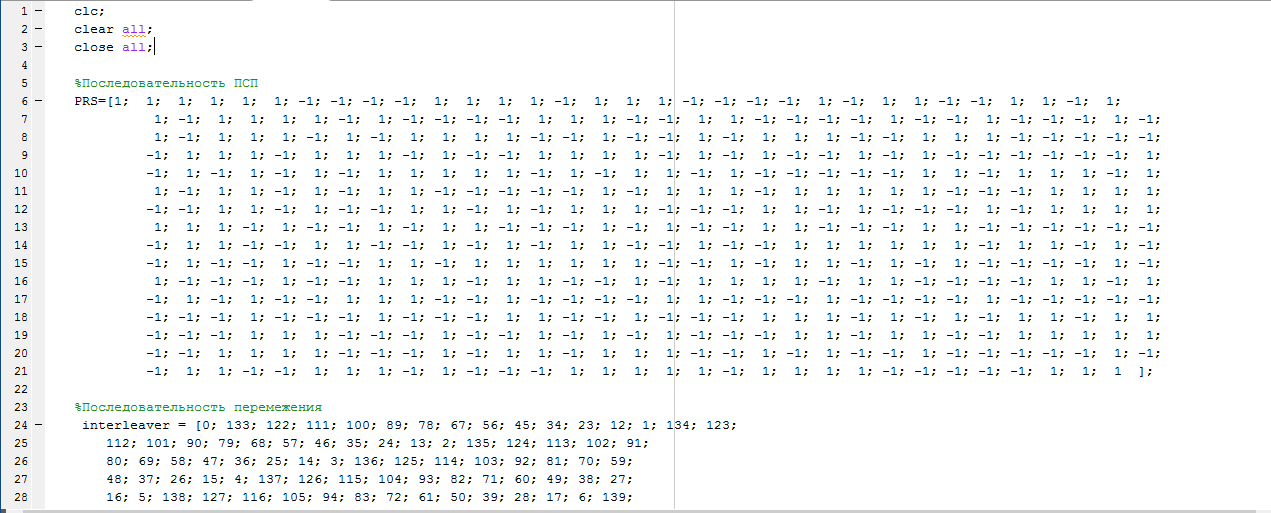
\includegraphics[width=0.9\linewidth]{part1}}
\caption{Код Matlab (часть 1))}
\end{figure}

\label{sec:part2}
%Рисунок 1
\begin{figure}[h!]
\center{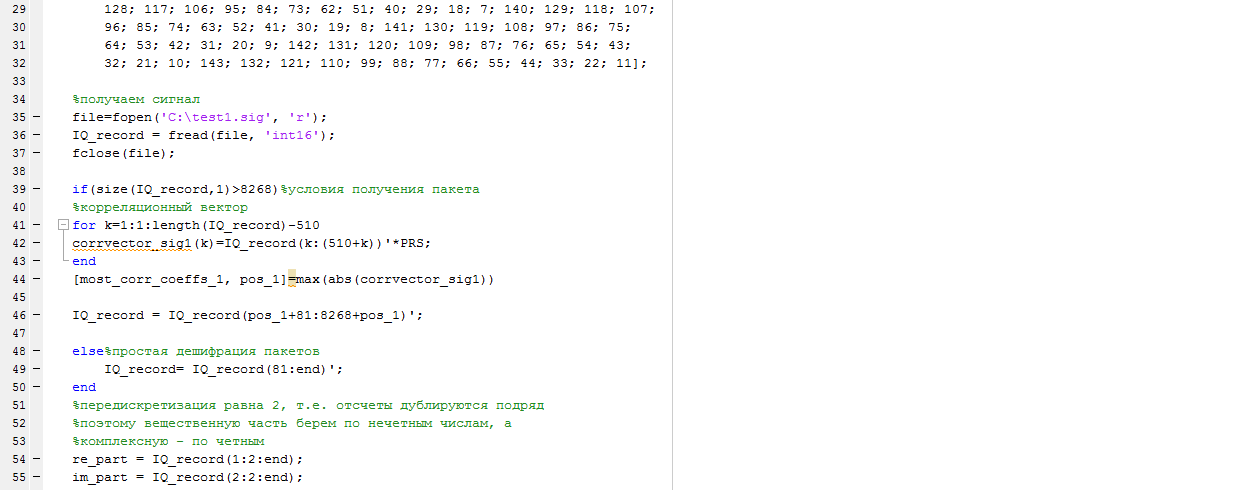
\includegraphics[width=0.9\linewidth]{part2}}
\caption{Код Matlab (часть 2))}
\end{figure}

\label{sec:part3}
%Рисунок 1
\begin{figure}[h!]
\center{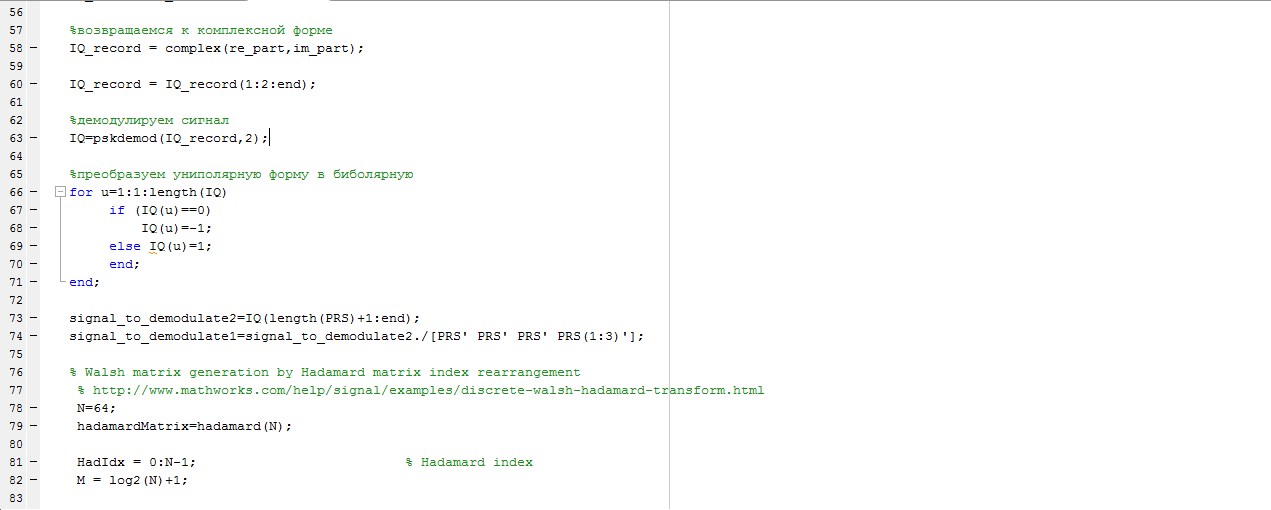
\includegraphics[width=0.9\linewidth]{part3}}
\caption{Код Matlab (часть 3))}
\end{figure}

\label{sec:part4}
%Рисунок 1
\begin{figure}[h!]
\center{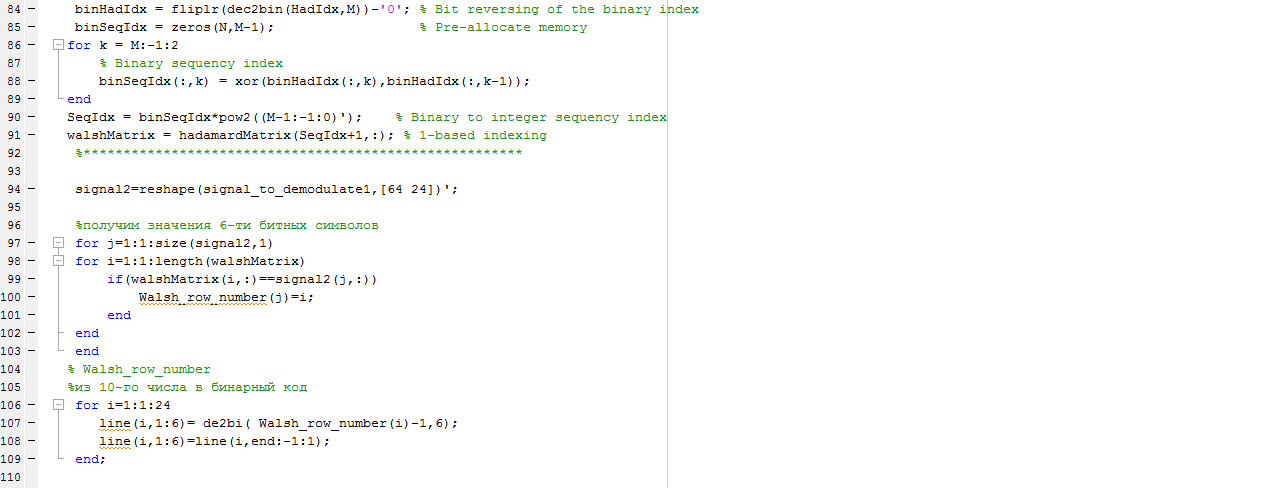
\includegraphics[width=0.9\linewidth]{part4}}
\caption{Код Matlab (часть 4))}
\end{figure}

\label{sec:part5}
%Рисунок 1
\begin{figure}[h!]
\center{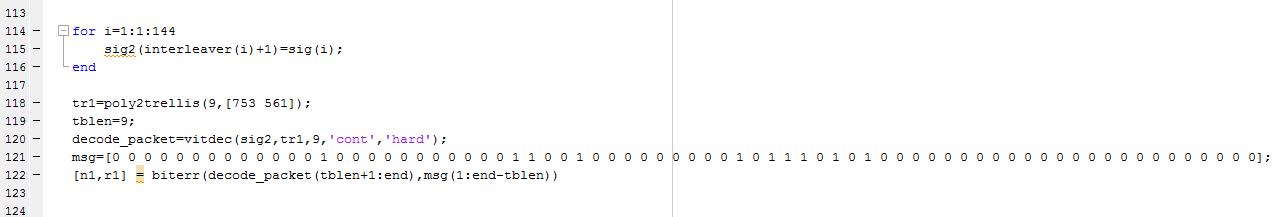
\includegraphics[width=0.9\linewidth]{part5}}
\caption{Код Matlab (часть 5))}
\end{figure}

\clearpage
\newpage

\section{Вывод}
\label{sec:afterWork}
В ходе данной работы была создана модель приемника. Были написан операции демодуляции, деперемежения и декодирования. 

\end{document}